\chapter{Algorthmen}
\label{cha:algorithmen}
% 7 Seiten

%supervised methoden: backpropagation
%unsupervised methoden: restricted boltzmann maschines, autoencoders, sparse coding model

Fokus: viele Daten, parallele Verarbeitung, viel Rechenpower

\section{Backpropagation}

\begin{figure}
	\centering
	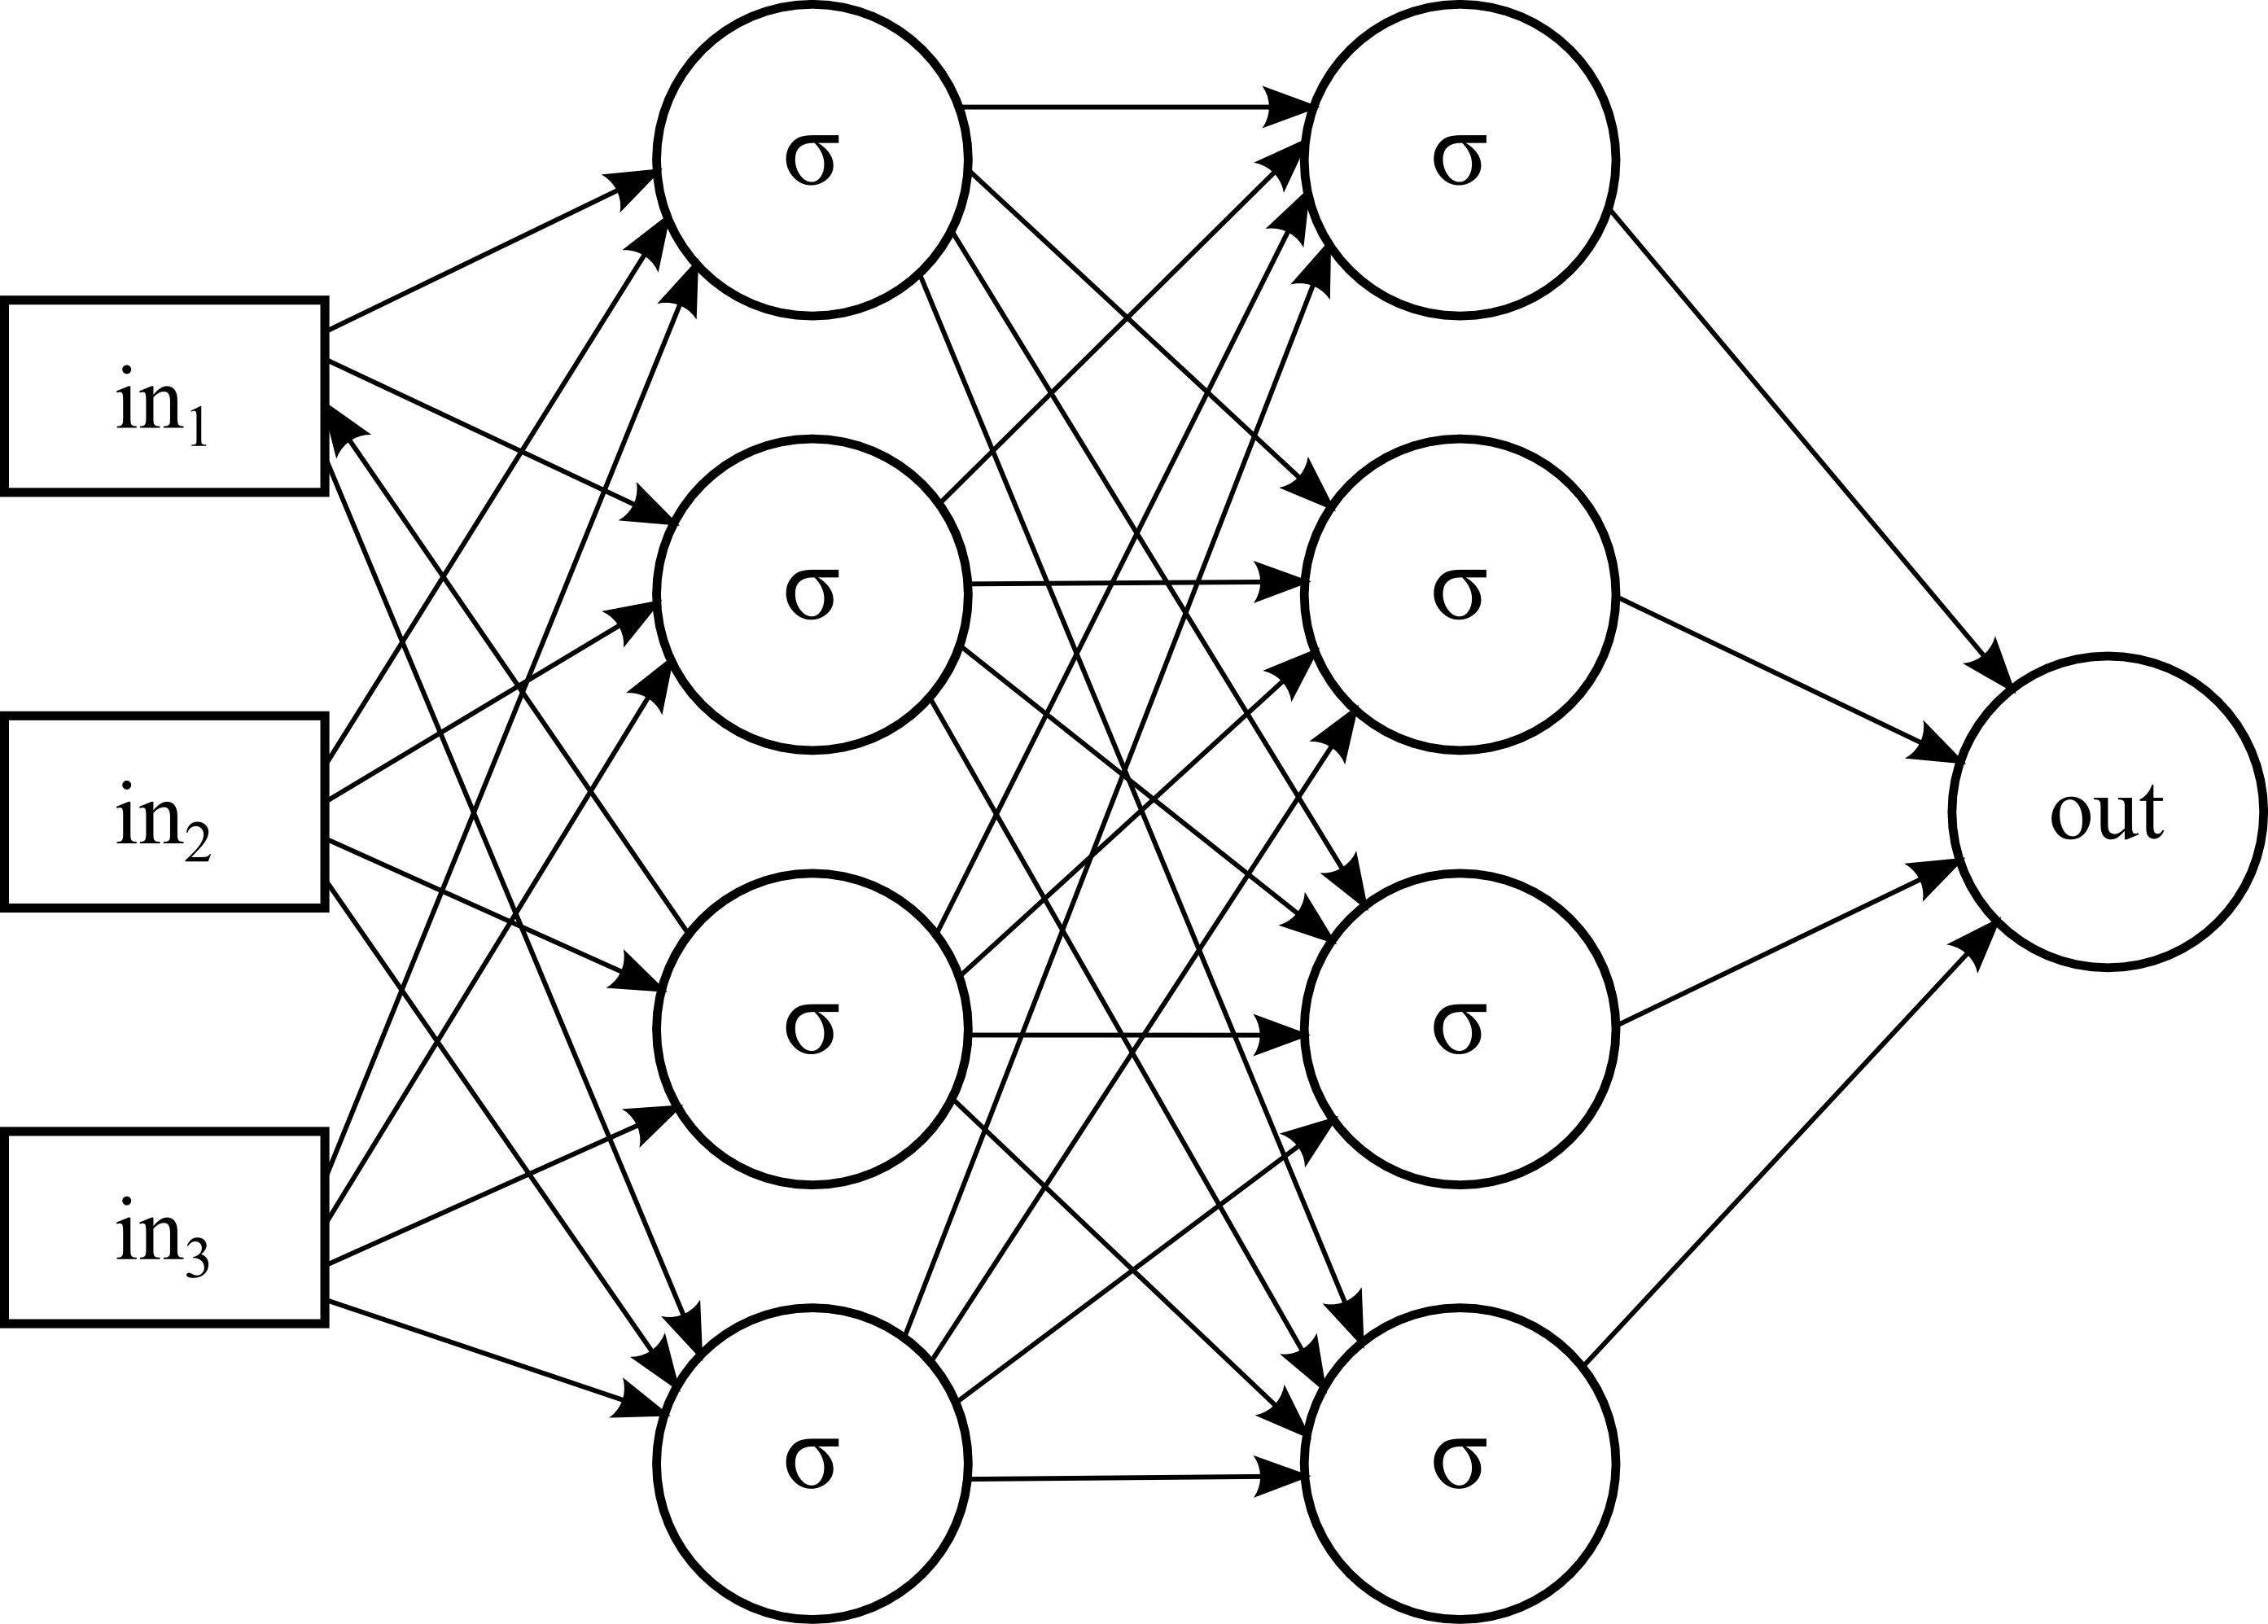
\includegraphics[scale=1]{images/net-for-bp.png}
	\caption{Ein Feedfowrward-Perzeptron}
	\label{fig:net-for-bp}
\end{figure}

Backpropagation ist ein überwachter Algorithmus zum Trainieren von vereinfachten neuronalen Netzen bei denen sich der Ausgang auf einfachem Weg berechnen werde kann, so genannten Feedforward-Perzeptrons, zu sehen in Abbildung \ref{fig:net-for-bp}. Überwacht bedeutet, dass das Netzwerk beim lernen anhand von kategorisierten Eingabedaten bestimmte Ausgabedaten zu errechnen. Der Fehler der Berechnung des Ausgangs wird beim Backpropagation-Algorithmus in die Adaptierung der Gewichte rückgeführt. Der Trainingsprozess beginnt mit zufälligen Gewichten und arbeitet in den folgenden Schritten:

\begin{enumerate}
\item Ausgang des Netzes für bestimmte Eingabedaten berechnen
\item Ausgang mit dem Sollwert vergleichen und daraus den Fehler errechnen
	$$error = \frac{1}{2}\sum_{k \in K}(out_k-target_k)^2$$
	\begin{center}\begin{tabular}{rclcrcl}
		$target$ & \dots & Fehler, der später Einfluss in die Gewichte nimmt\\
		$out$ & \dots & Wert den der Ausgang erreicht hat\\
		$target$ & \dots & Wert den der Ausgang erreichen sollte\\ 
		$K$ & \dots & Anzahl der Neuronen in der Ausgangsschicht\\
	\end{tabular}\end{center}
\item Gewichte je nach Größe des Fehlers anpassen
\end{enumerate}

Diese Schritte werden wiederholt, bis die Gewichte so angepasst wurden, das Eingabedaten möglichst gut klassifiziert werden können. Die Anpassung der Gewichte errechnet sich im wesentlichen anhand der Gradienten der Fehler und Gewichte. Zudem nimmt Schicht, vor der sich das jeweilige Gewicht befindet, Einfluss.

Wie der Name des Alogorithmus bereits verrät, wird der Fehler dabei im wesentlichen über eine mathematische Funktion in die Gewichte zurückgeführt. Diese Rückführung bringt zwei wesentliche Probleme mit sich:

\begin{itemize}
\item Lokale Minima
\item Überanpassung
\end{itemize}

Wird der Fehler geringer, so wird auch die Anpassung geringer. Befindet man sich auf dem Weg in ein lokales Optimum, so kann dieses sehr weit weg von dem globalen Optimum sein. Ist das Optimum entsprechend groß, so ist die Wahrscheinlichkeit, dass der Algorithmus in diesem Optimum hängen bleibt groß. Abhilfe können hier Verfahren wie der Bergsteigeralgorithmus oder Zufallsstreuungen in den Werten schaffen.

Die Überanpassung (eng. overfitting) 

\section{Resctricted Boltzmann Maschines}

\begin{figure}
	\centering
	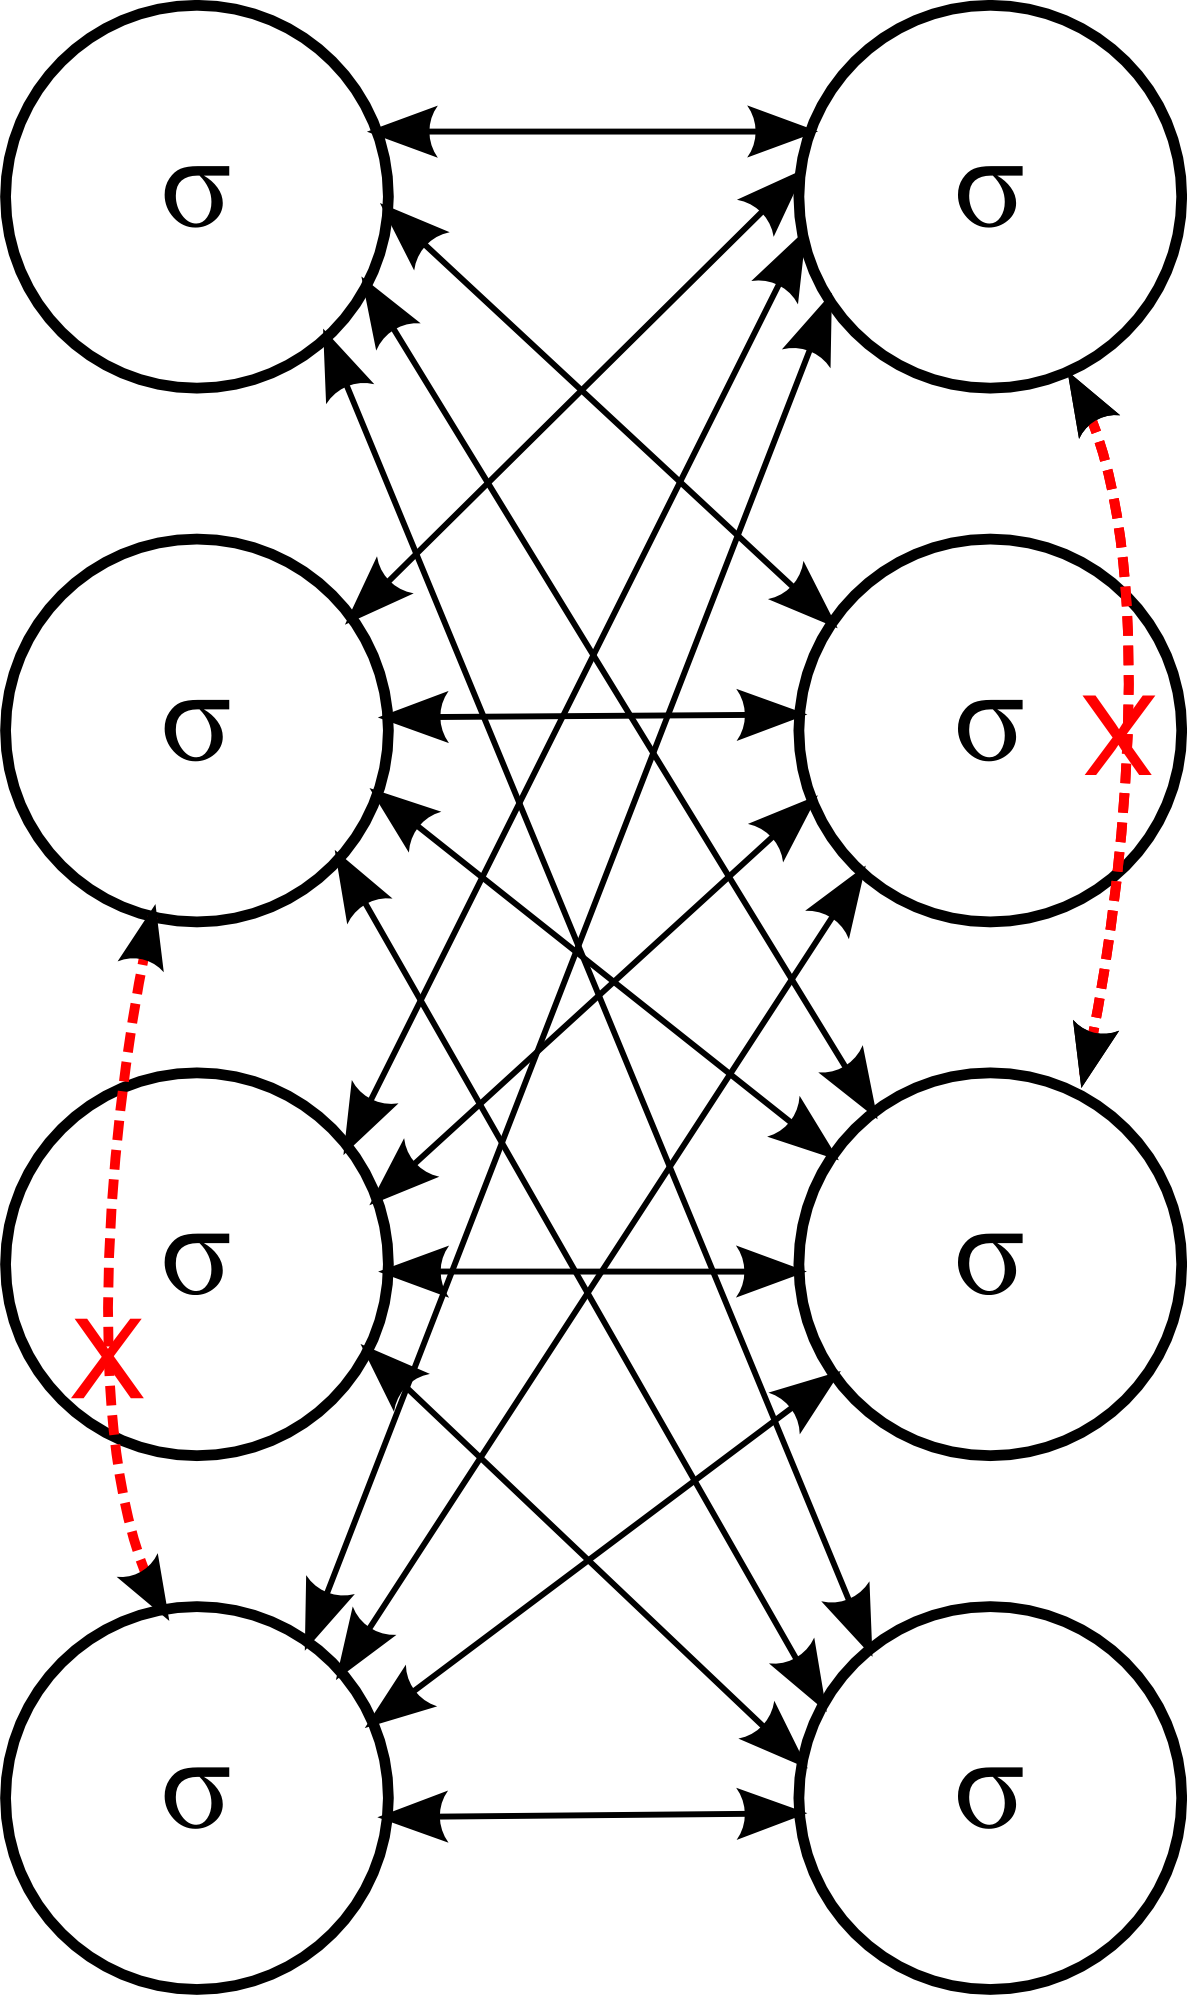
\includegraphics[scale=1]{images/rbm.png}
	\caption{Eine Restricted-Boltzmann-Maschine}
	\label{fig:rbm}
\end{figure}

Uneingeschränkte Neuronale-Netze sind schwierig und aufwendig zu trainieren. Restricted-Boltzmann-Maschines, im weiteren auch als RBMs bezeichnet, sind eingeschränkte neuronale Netzwerke. Wie in Abbildung \ref{fig:rbm} dargestellt, existieren hierbei nur Verbindungen zwischen aneinander liegenden Schichten. Das Modell erlaubt keine Verbindungen von Neuronen zu sich selbst und alle Verbindungen müssen gleichermaßen in beide Richtungen gehen. So lassen sich unter Festlegung der Werte einer Schicht direkt auf die nächste versteckte Schicht weiter gerechnet werden. RBMs arbeiten in der Regel mit bool'schen Werten, lassen sich durch Erweiterung aber auch mit anderen Zahlenräumen verwenden.

RMBs wurden bereits 1986 von Paul Smolensky \todo{ref} unter dem Namen Harmonium erfunden, fanden jedoch erst 1998, rund 10 Jahre später, durch die Entwicklung von effizienten Lernalgorithmen durch Geoffrey Hinton Anwendung.

Zum trainieren von RMBs existieren verschiedene Algorithmen, die meist auf dem Prinzip beruhen, die Gewichte so anzupassen, das das hin und her Rechen zwischen zwei Schichten wieder die Ausgangsdaten ergibt. Im folgenden wird der Algorithmus von Geoffrey Hinton \todo{reference}, der zugleich als der erste effizienten Lernalgorithmus für RMBs gesehen wird, erklärt. 

\subsection{Grundgedanke}

\begin{figure}%
\centering
\subfloat[Versteckte Schicht berechen]{\begin{minipage}{0.33\textwidth}\centering%
	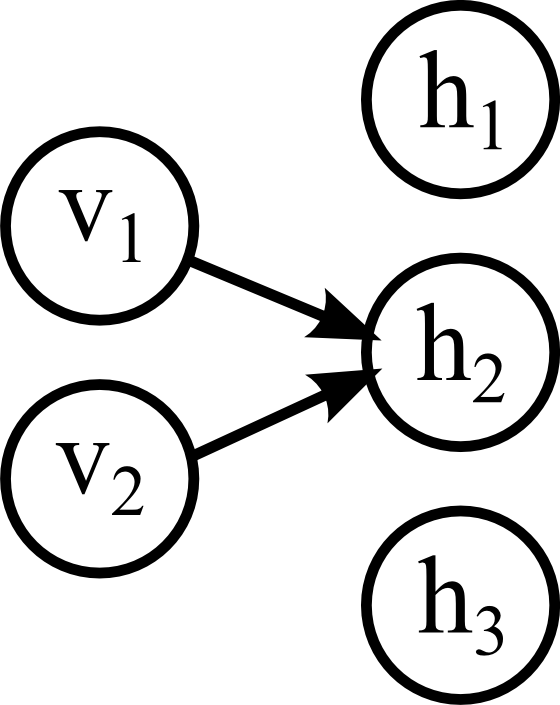
\includegraphics[scale=1]{images/rbm-step1.png}\end{minipage}}
\subfloat[Von der versteckten Schicht zurück rechnen]{\begin{minipage}{0.33\textwidth}\centering%
	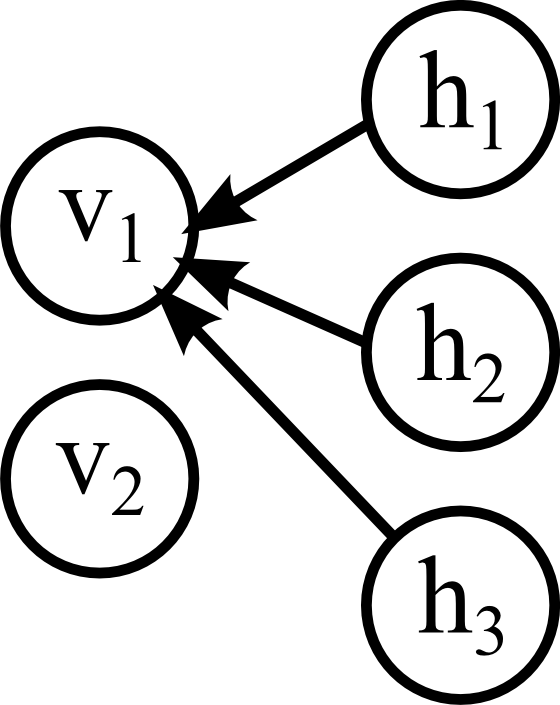
\includegraphics[scale=1]{images/rbm-step2.png}\end{minipage}}
\subfloat[Erneut die versteckte Schicht berechnen]{\begin{minipage}{0.33\textwidth}\centering%
	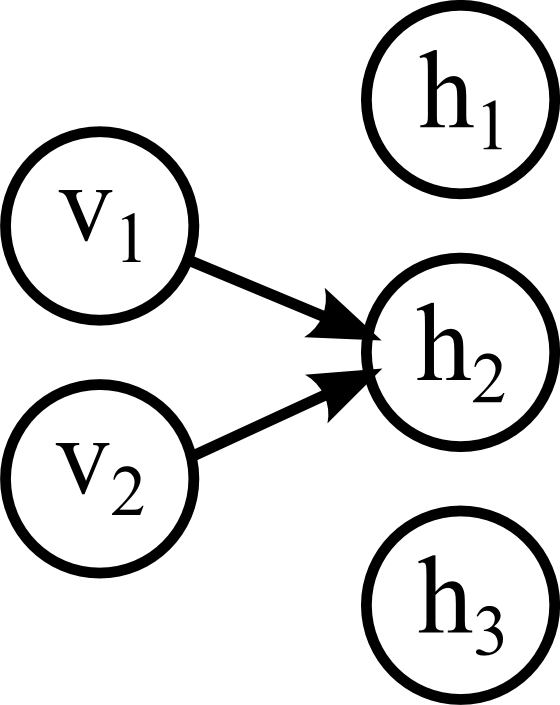
\includegraphics[scale=1]{images/rbm-step3.png}\end{minipage}}
\label{fig:rbm-steps}
\caption{Drei Berechnungsschritte zum Lernen von RBMs.}
\label{fig:rbm-steps}
\end{figure}

Sind die Werte einer Schicht fixiert, so kann einfach auf die nächste versteckte Schicht weiter gerechnet. Zu beginn werden wird ein Trainingsdatenset an die Eingänge angelegt und die folgenden Operationen, wie auch in Abbildung \ref{fig:rbm-steps} zu sehen, wiederholt ausgeführt:

\begin{enumerate}
\item Wahrscheinlichkeit für die versteckten Neuronen berechnen $$p(h_j=1) = \frac{1}{1+e^{-(b_j+\sum_{i}(v_i*w_{ij}))}}$$
\item Werte für die versteckte Schicht aus dem Mittelwert der Wahrscheinlichkeiten berechnen
\item Gradientenmatrix über das dyadische Produkt errechnen $$<v_ih_j> = v*y^T$$
\item Ausgehend von den errechneten versteckten Neuronen, zurück auf die sichtbare Schicht rechnen
\end{enumerate}

Wiederholt man die in der Liste angeführten Schritte sehr oft, so pendeln sich für die Neuronen Werte ein, die im wesentlichen vom Modell und den den Wahrscheinlichkeiten abhängen, jedoch sehr wenig mit den Eingangsdaten zu tun haben. Anhand der Gradientenmatrix des letzten Durchlaufes lässt sich jedoch eine Distanz zum gewünschten Modell herausfinden und so können die Gewichte wie folgt angepasst werden:
$$\Delta\omega_{ij} = \varepsilon (<v_ih_j>^0 -  <v_ih_j>^\infty)$$

Diese Art der Berechnung lieferte sehr gute Modelle. Durch die vielen Iterationen benötigt der Algorithmus sehr viel Rechenzeit und ist daher nicht praxistauglich. Zudem ist es schwierig festzustellen, wie viele Iterationen bis zum Einpendeln notwendig sind.

\subsection{Abkürzung}

Der oben genannte Algorithmus lässt sich in seiner Komplexität erheblich reduzieren, in dem die versteckte Schicht lediglich zwei mal berechnet wird. Geoffrey Hinton hat mit der Vereinfachung gezeigt, dass es möglich ist, bereits mit dem Vergleich der ersten und zweiten Gradientenmatrix möglich ist gute Ergebnisse zu erzielen. Diese Methode wird \emph{Contrastive Divergence} genannt.

Die Regel zur Anpassung der Gewichte lautet dann:
$$\Delta\omega_{ij} = \varepsilon (<v_ih_j>^0 -  <v_ih_j>^1)$$

\subsection{Begründung}

Der Grundgedanke von \emph{Contrastive Divergence} ist, dass das Modell mit Zufallsgewichten weg von den Eingabedaten, hin zu Daten die ihm besser gefallen, wandert. Wenn man erkennt wo hin das Modell die Daten ändert, kann man die Gewichte so adaptieren, dass dem Modell die Eingabedaten am besten gefallen.

\section{Eignung}

Das Modell besitzt nicht genügend Neuronen um alle Eingabedaten zu speichert und muss daher, um die Eingabedaten tatsächlich reproduzieren zu können, etwas aus den Eingabedaten lernen. Es eignet sich daher, um aussagekräftige Merkmale aus unkategorisierten Daten zu extrahieren.

\section{Autoencoders}

Autoencoders: Neuronales netz, mit backpropagation trainiert, das zumindest in einer Schicht weniger Neuronen als Eingangsparameter besitzt (bottelneck). Es wir so trainiert, dass der Ausgang dem Eingang entspricht. Steckt man vorne ein Bild hinein und das Netzwerk profezeit am Ausgang das gleiche Bild (mit allen Pixeln), so hat es offensichtlich etwas aus dem Bild gelernt und nicht nur alle Pixel durchgetunnelt (da Anzahl der neuronen kleiner als Anzahl der Pixel).
Es etsteht ein "Hash" für die Bilder - der wieder zurückgewandelt werden kann. Würde man es schaffen, beliebige Eingangsdaten sicher wiederherzustellen, so könnte man davon sprechen, dass das Netz das dahinter liegende System (die Natur) erlernt hat. Im weiteren könnte man so zum Beispiel von Bildern, Videos oder Audiospuren lediglich die Ergebnisse des Netztes speichern und die Eingangsdaten jederzeit widerherstellen. So ließen sich diverse Daten unter umständen erheblich komprimieren.

Füttert man solche Algorithmen mit Bildern und visualisiert die entstandenen Gewichte, so erkennt man, dass solche Algorithmen in erster Instanz meist Kanten und Farbintensitäten in Bildern finden. In der zweiten Schicht findet man einfache Kombinationen dieser Elemente und ab der dritten Schicht werden meist schon sehr brauchbare Neuronen zur vollständigen Objekterkennung ausgebildet.

Blockdiagramm mit mehreren Stufen (siehe Bilderkennung), zum Beispiel Matchen+Normalisieren, Matchen+Normalisieren, . . .


\section{Convolutional Neural Networks}
% als grundlage

\todo{super video, 10 minuten, erkärt das ganze thema: https://www.youtube.com/watch?v=n6hpQwq7Inw}
\todo{bild}
\todo[inline]{bild quelle: http://www.image-net.org/challenges/LSVRC/2012/supervision.pdf}
\todo[inline]{inhalt quelle: wiki, http://googlesystem.blogspot.co.at/2013/06/how-googles-image-recognition-works.html}

erlärung für bilder:
ein neuronales netzwerk, bestehend aus lauter kleineren gruppen an neuronen und vielen schichten. die kleinen Gruppen betrachten Ausschnitte des Bildes und überlappen in ihrer Anordnung. Durch den Blick auf den Ausschnitt eines Bildes wird das dahinter liegende Netzwerk in Teile geteilt und somit die Anzahl der Parameter und somit die Größe und benötigte Trainings und Rechenzeit stark verringert. Durch das Überlappen der einzelnen Bereiche wird berücksichtigt, dass ein späteres High-Level Feature nicht genau in einen Bereich trifft.
Das Überlappen gibt es auch zwischen den einzelnen Layern.
Convolutional networks können auch Layer enthalten, die mehrere Ausgänge von neuronen kombinieren, so genannte polling layer.

Dieser Typ von Netzwerk ist bereits 1980 \todo{paper Kunihiko fukushima}, wurde in den folgenden Jahrzehnten optimiert und erlebte einen Aufschwung durch eine Implementierung auf einer GPU \todo{Dan Ciresan}. Nach weiteren Optimierungen in den vergangen Jahren wurde der Algorithmus unter anderem für ein Projekt von Google \todo{google paper finden} eingesetzt, das nicht zuletzt das so genannte face-neuron ausprägte.

convolution: operation that expresses the amount of overlap with another function
image preprozessing mit gabor filters, erkennt kanten in alle richtungen



\section{betrachtung als restricted bolzman maschine}


